
open source ones, matlab toolkit, with its latest implementation

Talk about ligand molecule orientation sensor, cite pygbe

\item{\textit{Ligand molecule orientation} Where the ligand molecule absorption is dominated
by electrostatic effects, was study in previous work \cite{CooperClementiBarba2015}
using the biomolecular electrostatics \pygbe application \cite{CooperETal2016}}


# 2 - What is UNknown, limitations and gaps

Unkown: relation between high dependance on sensitivity on distance in LSPR biosensors.
Find structural details of analyte and nanoparticle, and the relative position between them.

Gap: study this using fast, free-software dependencies and open source computer
simulations. 

limitations - private are expensible and not accessible, 
              matlab not free, 
              no grid convergence analysis or error study, 
              no reproducible framework 
              problem size, geometry, and computation time




# 3 - Burning question, experimental approach, why ours is new and diff (fill the gap)

SOlve this problem with pygbe? yes

long wavelength limit we don't need full Maxwell eq, we can approach it using
electrostatics.

\item{\textit{Localized surface plasmon resonance (LSPR) biosensor} This type
of biosensors measure the shift of plasmon resonace frequency in metallic nanoparticles
when a target molecules binds to it. LSPR is an optical effect, but electrostatics 
makes a good approximation in the long-wavelength limit. In this work we use
PyGBe's approach to study how the LSPR response changes in the presence of a 
biomolecule.}


\pygbe most recent 
application \cite{ClementiETal2017} tends to bridge that gap providing via
simulations, insights to guide the reasearch process. 

The latest release of \pygbe
extends the software to nanoplasmonics treating localized surface plasmon 
resonance (LSPR) quasi-statically \cite{MayergoyzZhang2007}.

Mentions that uses treecode, gmres and GPU. 

The software \footnote{\url{https://github.com/barbagroup/pygbe}} is shared 
under the BSD 3-clause license and the development repository is available on 
Github.







\begin{figure}[h] %  figure placement: here, top, bottom, or page
   \centering
   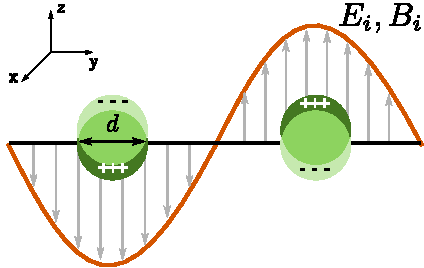
\includegraphics[width=0.35\textwidth]{lspr.pdf} 
   \caption{Localized Surface Plasmon Resonance (LSPR) scheme. LSPR is an 
            optical phenomenon that ocurrs when light shines on conductive 
            nanoparticles that are smaller than the wavelength of the incident 
            light. The free electrons on the surface of the nanoparticle are 
            excited by the incoming electric field oscillating with it and 
            creating plasmons \textcolor{blue}{this figure is from another paper. We should redo it or cite.}.\textcolor{red}{I modify some things of the original picture, do we still need to cite?}}
   \label{fig:lspr}
\end{figure}




